%* Overview of LHC and experiments at the interaction points
The Large Hadron Collider \cite{LHC:LHC} (LHC) is a two-ring proton-proton and Pb-Pb ion collider installed into the 27km long LEP tunnel at CERN. The primary discovery goal of the LHC was the observation of the Higgs boson which was achieved in July 2012 \cite{Atlas:higgs}. The LHC has two high-luminosity experiments, ATLAS \cite{Atlas:design} and CMS \cite{LHC:CMS} with a design peak luminosity of $10^{34}\text{cm}^{-2}\text{s}^{-1}$, in addition to TOTEM \cite{LHC:TOTEM}, LHCb \cite{LHC:LHCb}, and ALICE \cite{LHC:ALICE}. 

%showing the different beam Insertion Regions (IR) corresponding to 
The proton source for the LHC is a bottle of hydrogen gas. The hydrogen is ionised by an electric field before they are accelerated to around 50\MeV by Linac 2. The Proton Synchrotron (PS) PS accelerates protons to 25\GeV and provides them as bunches with a 25ns spacing to the Super Proton Synchrotron (SPS). The SPS accelerates the bunches to an energy of 450\GeV. The acceleration of proton bunches in the LHC itself is achieved through the radiofrequency (RF) system. The RF system is comprised of 16 RF cavities housed in 4 cryomodules. Each RF cavity delivers an oscillating longitudinal electric field of 5MV/m, delivering an accelerating voltage of 2MV at a frequency of 400MHz. The RF cavities serve two primary purposes, first to accelerate the protons with every pass of the RF system, and second to group the packets of  protons from the PS into even tighter bunches, to ensure a high luminosity at the collision points. The proton injection is timed such that the center of a packet of protons is located just after the oscillating field maximum. Hence, protons just before the center of the bunch (closer to the field maximum) will be accelerated more than protons just after the center of the bunch (further from the field maximum). This results in protons away from the center of the bunch to be moved towards the center, creating stable, tight, bunches. The number of possible stable bunches ($h$) is therefore equal to the number of possible synchronised protons. A proton is synchronised if the RF frequency ($f_{\text{RF}}$) is an integer multiple of the revolution frequency ($f_{\text{rev}}$)
\begin{equation}
    f_{\text{RF}}=h\times f_{\text{rev}}.
\end{equation}
Therefore dividing the two frequencies gives the number of possible bunches. With $f_{\text{rev}}=c/27$km and $f_{\text{RF}}=400$MHz, this gives the value of $h$ as approximately 35640. These are called RF buckets. Not every RF bucket is filled, and the number of occupied buckets in the LHC is 2808. Each bunch contains $\sim \num{1.15e11}$ protons \cite{LHC:design,LHC:acceleratorspedestrians,LHC:rfcavities}. A schematic of the CERN accelerator complex is shown in Figure \ref{fig:LHC:ccc}.
\begin{figure}[t]
    \centering
    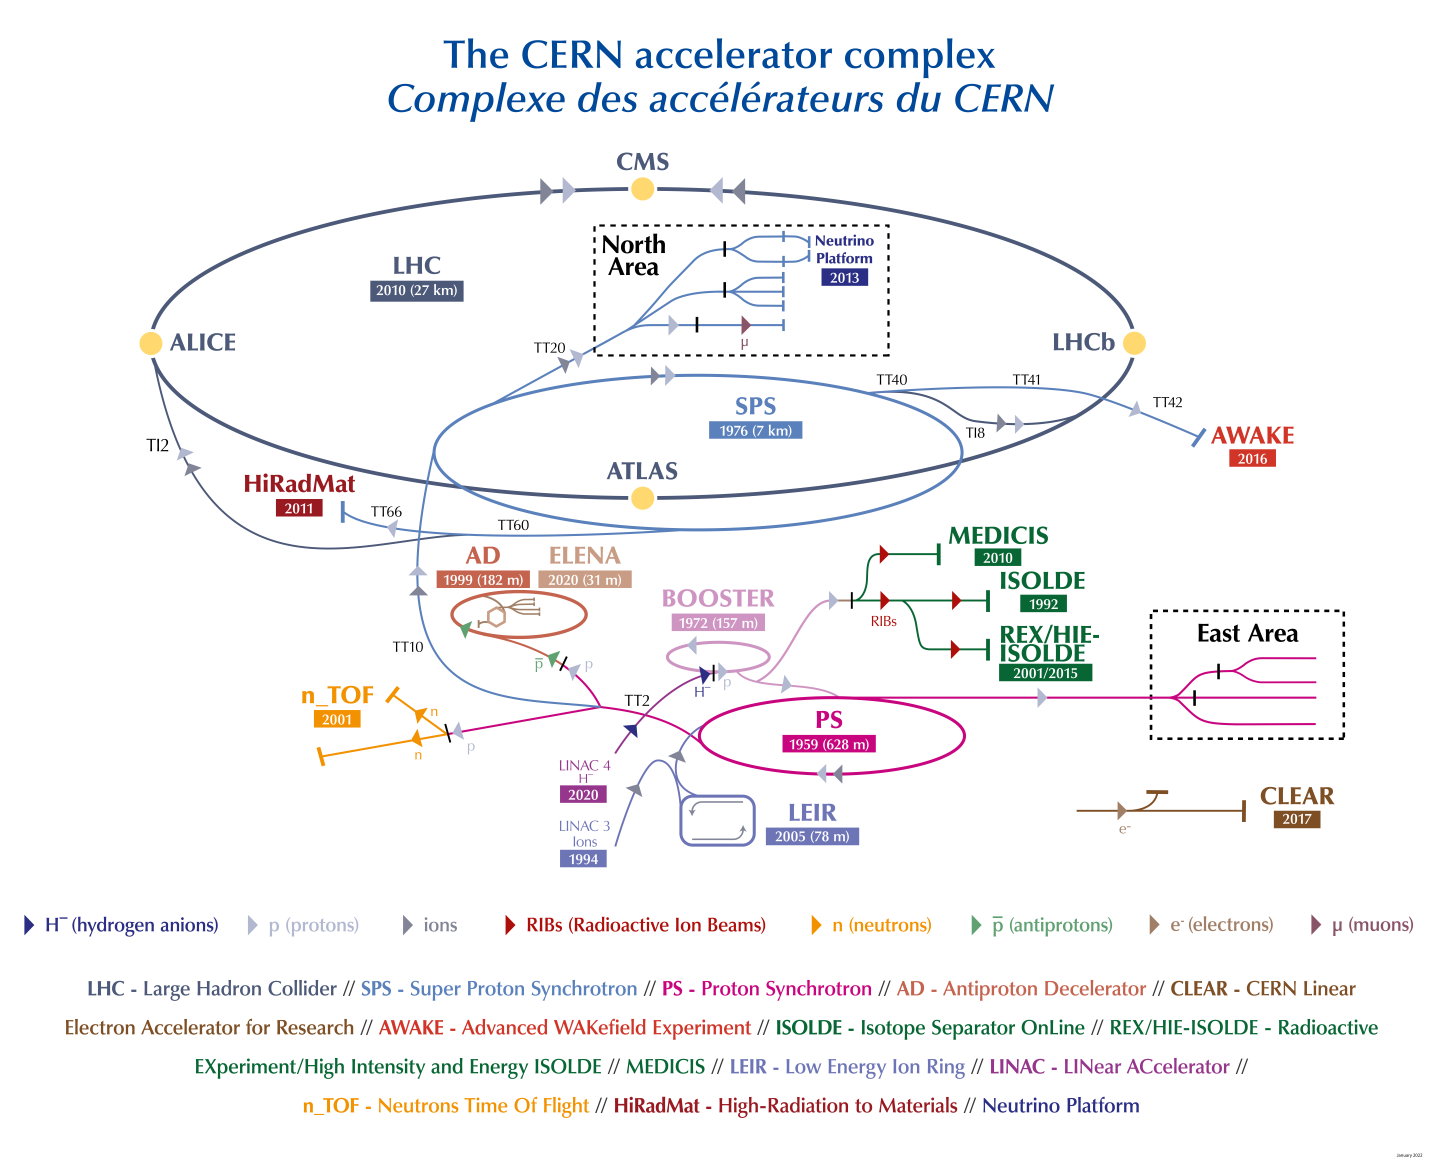
\includegraphics[width=\textwidth]{plots/lhc/CCC-v2022.png}
    \caption{The CERN accelerator complex. Figure taken from \cite{LHC:CCC}.\label{fig:LHC:ccc}}
\end{figure}
As protons carry electric charge, the particle beam will naturally diverge. In the curved sections of the LHC (arcs), the beam must be focused such that its width and height are constrained to be within the vacuum chamber. At the interaction Points (IPs), to enhance the interaction probability for each bunch crossing, the beams are focussed to a size of 16$\mu$m in the $x-y$ plane for CMS and ATLAS. The focussing in the arcs is achieved by collections of superconducting quadrupole, dipole, and other multipole magnets organised into twenty-three LHC cells per arc, resulting in a total of 858 quadrupoles and 1232 dipoles. For the 1232 superconducting dipoles to operate reliably at the 8.33T magnetic field required for 7 TeV beams, the magnet system must operate in a bath of superfluid helium at a temperature of 1.9K. Dispersion suppressors, comprised of four quadrupoles separated by two dipole magnets, are located at the boundaries between the beam insertion regions (IRs) and the arcs, and reduce the machine dispersion (momentum spread of particles within a bunch). Reducing the machine dispersion at the IPs to zero requires two additional quadrupole magnets at each side of the arc. The focusing of the bunches at the IP is achieved using 8 sets of superconducting ``inner triplet'' magnets \cite{LHC:magnets1,LHC:magnets2,LHC:design}. 
%
%\begin{figure}[htb]
%    \centering
%    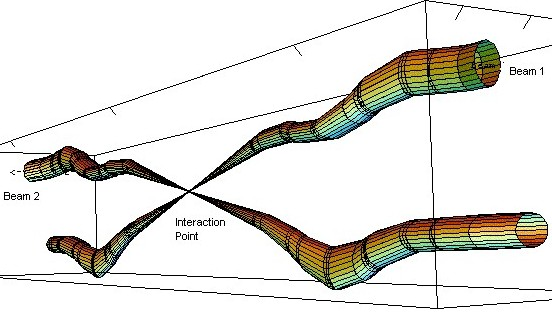
\includegraphics[width=0.6\textwidth]{plots/lhc/interactionpoint_lhc.jpg}
%    \caption{The geometrical configuration of beams leading up to the IPs at the LHC. Figure from \cite{LHC:beams}}
%    \label{fig:lhc_ip}
%\end{figure}
%Before protons reach the LHC, they are accelerated through the LHC injection chain which is comprised of the Proton Synchrotron (PS) and Super Proton Synchrotron (SPS). The PS accelerates protons to 25\GeV and provides them as packets with a 25ns spacing to the SPS. The SPS then accelerates the packets to an energy of 450\GeV. The acceleration of proton packets in the LHC itself is achieved through the radiofrequency (RF) system. The RF system is comprised of 16 RF cavities housed in 4 cryomodules located in LSS4 of the LHC ring. Each RF cavity delivers an oscillating longitudinal electric field of 5MV/m delivering an accelerating voltage of 2MV at a frequency of 400MHz. The RF cavities serve two primary purposes, first to accelerate the protons with every pass of the RF system, and second to group the packets of  protons from the PS into even tighter bunches to ensure a high luminosity at the collision points. The grouping into tight bunches happens because the protons tend to oscillate around those synchronised with the RF frequency. The proton injection is timed such that the center of a packet of protons is located just after the oscillating field maximum. Hence protons just before the maximum will accelerate towards the center, and protons after the maximum will decelerate towards the center, creating stable bunches. The number of possible stable bunches ($h$) is therefore equal to the number of possible synchronised protons. A proton is synchronised if the RF frequency is an integer multiple of the revolution frequency:
%\begin{equation}
%    f_{\text{RF}}=h\times f_{\text{rev}},\hspace{5pt} h=\frac{f_{\text{RF}}}{f_{\text{ref}}}.
%\end{equation}
%Substituting the protons revolution frequency of $c/27\text{km}$ and substituting the RF frequency of 400MHz, gives the value of $h\approx35640$, which is number of possible bunches. These are called RF buckets. Not every RF bucket is filled, and the number of occupied buckets in the LHC is 2808 \cite{LHC:design}\cite{LHC:acceleratorspedestrians}\cite{LHC:rfcavities}.
%only see the maximum accelerating voltage at the gap at an interval equal to an integer multiple of the 400MHz electric field frequency, and %Protons are initially injected into the cavities at an energy of 450\GeV after passing through the pre-accelerator known as the Super Proton Synchrotron (SPS). % Since there are 8 RF cavities, with every pass a proton receives 2MV$\times$8=16MeV of energy. Assuming protons travel at the speed of light, and taking the circumference of the LHC ring as 26669m, means that there are 11245 passes per second, resulting in $11245\times16\MeV=0.18\TeV$  %The RF cavities are responsible for bringing the beam energy up to 6.5 TeV (6.8TeV in run3). The frequency of the RF cavities is tuned to around 400MHz, 
%Now include some info about number of bunch crossings/second, number of interactions per second, primary verticles vs pileup vertices, etc.

\clearpage
\section{Luminosity and cross-sections}

The number of scattering events $N$ in a given amount of time is called the event rate, and depends on the geometric nature of the beam, and on the individual $pp$ interactions. For a given bunch crossing, each proton has an associated cross-sectional area where if another proton is within this, they may interact. It follows that the scattering probability is related to a quantity with units of area known as the \textit{scattering cross-section}, $\sigma$. $N$ is directly related to $\sigma$ and must satisfy
\begin{equation}\label{eq:instlumi}
    \frac{\mathrm{d}N}{\mathrm{d}t}=\mathcal{L}(t)\sigma,
\end{equation}
which defines the quantity known as the \textit{instantaneous luminosity} $\mathcal{L}(t)$. Integrating this equation yields the integrated luminosity $L$
\begin{equation}
    L=\int_{0}^{T}\mathcal{L}\mathrm{d}t,
\end{equation}
which is a measure of how much data has been taken in time $T$. Equation \ref{eq:instlumi} can be written in terms of $L$ as \cite{Buckley:PCP}
\begin{equation}
    N=\sigma L.
\end{equation}
The instantaneous luminosity depends on a number of beam parameters, and is given by
\begin{equation} \label{eq:lumi_1}
    \mathcal{L}(t)=\frac{N_b^2n_bf_{rev}\gamma_r}{4\pi\epsilon_n\beta^*},
\end{equation}
where $N_b$ is the number of particles per bunch, $n_b$ the number of bunches per beam, $f_{\text{rev}}$ the revolution frequency, $\gamma_r$ the relativistic gamma factor, $\epsilon_n$ the normalized transverse beam emittance (this reflects the beam quality, and is roughly defined as the smallest opening the beam can be squeezed through), $\beta^*$ the beta function (the width of the beam, squared, divided by the emittance) at the collision point and $F$ a geometric luminosity reduction factor. The linear dependence on $\gamma_r$ and square dependence on $N_b$ implies that a large luminosity requires beams of high energy and high intensity. Separate dipole magnetic fields and vacuum systems are required for the two beams, as both beams contain positively charged protons. At the IRs the two beams share a common 126m (for ATLAS and CMS) long beam pipe.

The luminosity in the LHC is not constant over a physics run. The beam intensities and emittances of the circulating beams degrade primarily due to the collisions themselves, leading to a decay in the luminosity. This is quantified with the luminosity lifetime, $\tau_L$. 

The expected integrated luminosity of the LHC of a luminosity run is given by
\begin{equation}
    L=L_0\tau_L(1-e^{-T_{\text{run}}/\tau_L}),
\end{equation}
where the assumption is made that the time for beam injection, ramping up the beam energy, ramping down the magnets, and programmed main systems checks total a turnaround time of $T_{\text{turnaround}}\approx 70\text{min}$. Assuming that the LHC is taking data 200 days a year for an optimum run time of 12h, the total maximum luminosity per year is about 120\invfb \cite{LHC:design}.

The Run-2 total integrated luminosity is shown in Figure \ref{fig:LHC:intlumi}. The Run-2 integrated luminosity recorded by ATLAS with good data quality is $140.1\infb$ \cite{LHC:atlaslumi}.

\begin{figure}[t]
    \centering
    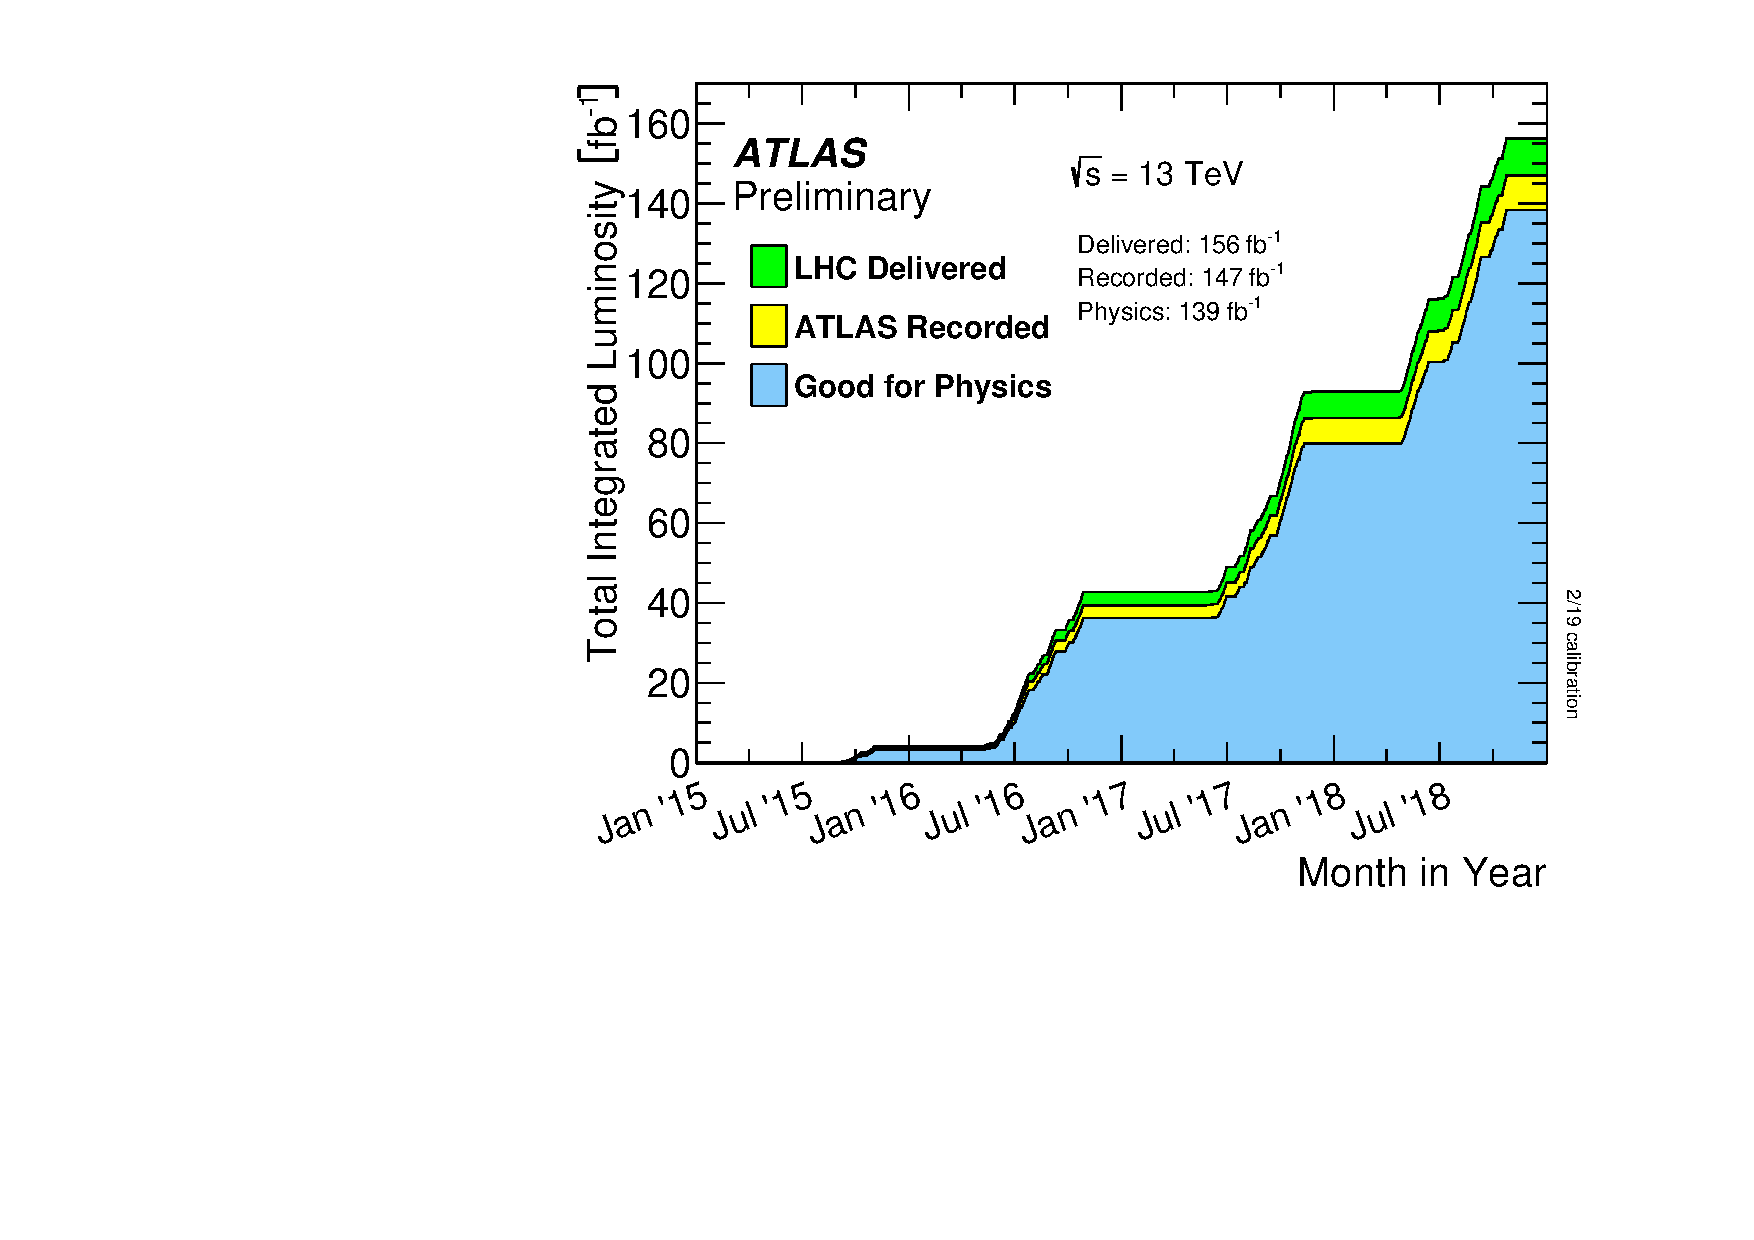
\includegraphics[width=\textwidth]{plots/lhc/intlumivstimeRun2DQall.pdf}
    \caption{The total integrated luminosity for Run-2 versus time. The green curve shows the luminosity delivered to ATLAS by the LHC. The yellow curve shows the luminosity recorded by ATLAS. The blue curve shows the luminosity of the dataset certified to be good data quality. Since this plot has been produced, the most accurate assessment of the total integrated luminosity certified good for physics has been updated to 140\infb \cite{LHC:atlaslumi}. Figure from \cite{LHC:deliveredlumi}.\label{fig:LHC:intlumi}}
\end{figure}

\clearpage
\section{Pile-up}

All LHC analyses need to contend with the harsh experimental conditions which come about due to the very large number of interactions per bunch crossing. The mean number of interactions per bunch-crossing (averaged over luminosity) $\langle\mu\rangle$ in Run-2 was $\langle\mu\rangle = 33.7$. The largest momentum transfer happens in the primary hard scatter interaction, all other secondary interactions are referred to as pile-up interactions and consist mainly of soft-QCD processes. There are two types of pile-up. In-time pileup refers to $pp$ collisions from the same bunch-crossing as the interaction of interest, whereas out-of-time pileup refers to $pp$ collisions occurring in bunch-crossings just before and after the interaction of interest. 

Pileup is responsible for a large number of soft hadrons distributed throughout the detector. Therefore the reconstruction of jets and Missing Transverse Energy (MET) are especially effected. Without pileup mitigation techniques, the energies of jets will in general be overestimated, and spurious jets not associated with the hard scatter will be included in the event leading to changes in the MET measurement. In addition to these biases, pileup also results in the degradation of the resolution of reconstructed quantities. The reason for this is that the pileup activity itself is not a fixed quantity, which therefore results in fluctuations of the bias due to pileup. The challenges associated with pileup in the context of object reconstruction is discussed in more detail in Section \ref{sec:objreco} \cite{Buckley:PCP,LHC:pileup}.
